% Copyright 2003 by Till Tantau <tantau@cs.tu-berlin.de>.
%
% This program can be redistributed and/or modified under the terms
% of the LaTeX Project Public License Distributed from CTAN
% archives in directory macros/latex/base/lppl.txt.


\section{Design Principles}

This section describes the basic layer of \pgfname. This layer is
build on top of the system layer. Whereas the system layer just
provides the absolute minimum for drawing graphics, the basic
layer provides numerous commands that make it possible to create
sophisticated graphics easily and also quickly.

The basic layer does not provide a convenient syntax for describing
graphics, which is left to frontends like \tikzname. For this reason, the
basic layer is typically used only by ``other programs.'' For example,
the \textsc{beamer} package used the basic layer extensively, but does
not need a convenient input syntax. Rather, speed and flexibility are
needed when \textsc{beamer} creates graphics.

The following basic design principles underlie the basic layer:
\begin{enumerate}
\item Structuring into a core and several optional packages.
\item Consistently named \TeX\ macros for all graphics commands.
\item Path-centered description of graphics.
\item Coordinate transformation system.
\end{enumerate}



\subsection{Core and Optional Packages}

The basic layer consists of a \emph{core package}, called |pgfcore|,
which provides the most basic commands, and several optional package
like |pgfbaseshade| that offer more special-purpose commands.

You can include the core by saying |\usepackage{pgfcore}| or, as a
plain \TeX\ user, |\input pgfcore.tex|.

The following optional packages are provided by the basic layer:
\begin{itemize}
\item
  |pgfbaseplot| provides commands for plotting functions.
\item
  |pgfbaseshapes| provides commands for drawing shapes and
  nodes.   
\item
  |pgfbaseimage| provides commands for including external
  images. The |graphicx| package does a much better job at this than
  the |pgfbaseimage| package does, so you should normally use
  |\includegraphics| and not |\pgfimage|. However, in some situations
  (like when masking is needed or when plain \TeX\ is used) this
  package is needed.
\end{itemize}

If you say |\usepackage{pgf}| or |\input pgf.tex|, all of the optional
packages are loaded (as well as the core and the system layer).


\subsection{Communicating with the Basic Layer via Macros}

In order to ``communicate'' with the basic layer you use long
sequences of commands that start with |\pgf|. You are only allowed to
give these commands inside a |{pgfpicture}| environment. However, it
is possible to ``do other things'' between the commands. For example,
you might use one command to move to a certain point, then have a
complicated computation of the next point, and then move there.

\begin{codeexample}[]
\newdimen\myypos
\begin{pgfpicture}
  \pgfpathmoveto{\pgfpoint{0cm}{\myypos}}
  \pgfpathlineto{\pgfpoint{1cm}{\myypos}}
  \advance \myypos by 1cm
  \pgfpathlineto{\pgfpoint{1cm}{\myypos}}
  \pgfpathclose
  \pgfusepath{stroke}
\end{pgfpicture}
\end{codeexample}

The following naming conventions are used in the basic layer:

\begin{enumerate}
\item
  All commands and environments start with |pgf|.
\item
  All commands that specify a point (a coordinate) start with |\pgfpoint|.
\item
  All commands the extend the current path start with |\pgfpath|.
\item
  All commands that set/change a graphics parameter start with |\pgfset|.
\item
  All commands that use a previously declared object (like a path,
  image or shading) start with |\pgfuse|.
\item
  All commands having to do with coordinate transformations start with
  |\pgftransform|. 
\item
  All commands having to do with declaring arrows start with |\pgfarrows|.
\item
  All commands for ``quickly'' extending or drawing a path start with
  |\pgfpathq| or |\pgfusepathq|.
\end{enumerate}


\subsection{Path-Centered Approach}

In \pgfname, the most important entity is the \emph{path}. All
graphics are composed of numerous paths that can be stroked,
filled, shaded, or clipped against. Paths can be closed or open, they
can self-intersect and consist of unconnected parts.

Paths are first \emph{constructed} and then \emph{used}. In order to
construct a path, you can use commands starting with |\pgfpath|. Each
time such a command is called, the current path is extended in some
way.

Once a path has been completely constructed, you can use it using the
command |\pgfusepath|. Depending on the parameters given to this
command, the path will be stroked (drawn) or filled or subsequent
drawings will be clipped against this path.




\subsection{Coordinate Versus Canvas Transformations}

\label{section-design-transformations}

\pgfname\ provides two transformation systems: \pgfname's own
\emph{coordinate} transformation matrix and \pdf\ or PostScript's
\emph{canvas} transformation matrix. These two systems are quite
different. Whereas a scaling by a factor of, say, $2$ of the canvas
causes \emph{everything} to be scaled by this factor (including
the thickness of lines and text), a scaling of two in the coordinate 
system causes only the \emph{coordinates} to be scaled, but not the
line width nor text.

By default, all transformations only apply to the coordinate
transformation system. However, using the command |\pgflowlevel|
it is possible to apply a transformation to the canvas.

Coordinate transformations are often preferable over canvas
transformations. Text and lines that are transformed using canvas 
transformations suffer from differing sizes and lines whose thickness 
differs depending on whether the line is horizontal or vertical. To
appreciate the difference, consider the following two ``circles'' both
of which have been scaled in the $x$-direction by a factor of $3$ and
by a factor of $0.5$ in the $y$-direction. The left circle uses a
canvas transformation, the right uses \pgfname's coordinate
transformation (some viewers will render the left graphic incorrectly
since they do no apply the low-level transformation the way they
should):  

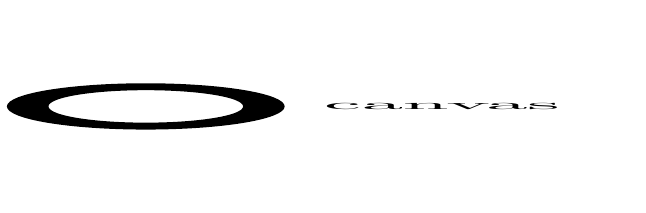
\begin{tikzpicture}[line width=5pt]
  \useasboundingbox (-1.5,-1) rectangle (6,1);
  
  \begin{scope}
    \pgflowlevel{\pgftransformxscale{3}}
    \pgflowlevel{\pgftransformyscale{.5}}

    \draw (0,0) circle (0.5cm);
    \draw (.55cm,0pt) node[right] {canvas};
  \end{scope}
  \begin{scope}[xshift=9cm,xscale=3,yscale=.5]
    \draw (0,0) circle (0.5cm);
    \draw (.55cm,0pt) node[right] {coordinate};
  \end{scope}
\end{tikzpicture}

